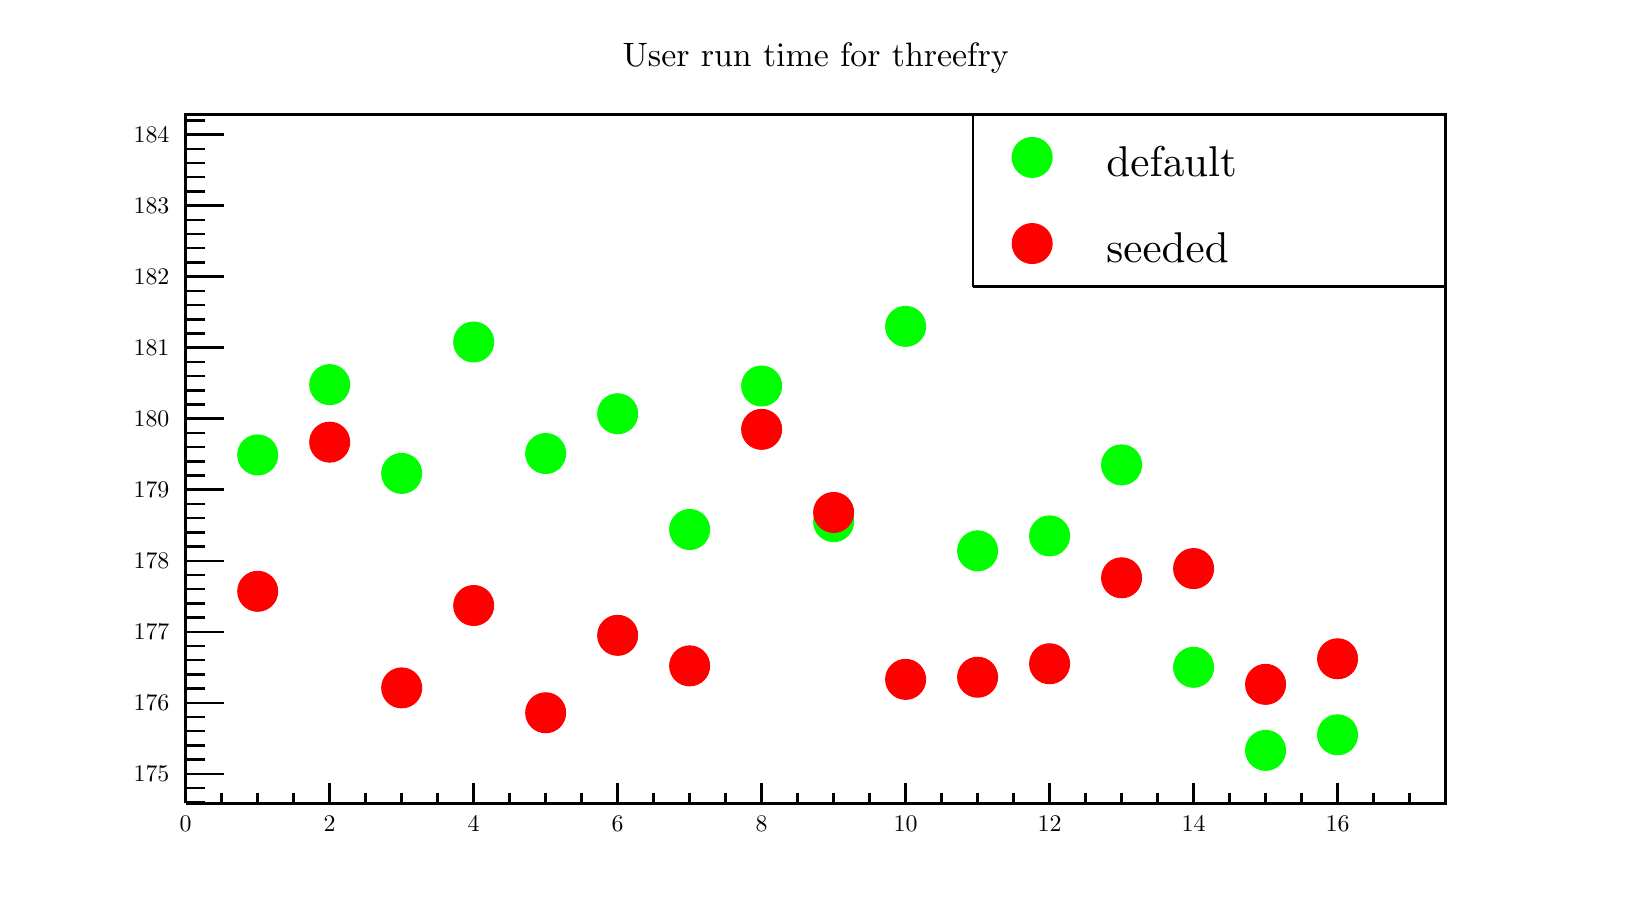
\begin{tikzpicture}
\pgfdeclareplotmark{cross} {
\pgfpathmoveto{\pgfpoint{-0.3\pgfplotmarksize}{\pgfplotmarksize}}
\pgfpathlineto{\pgfpoint{+0.3\pgfplotmarksize}{\pgfplotmarksize}}
\pgfpathlineto{\pgfpoint{+0.3\pgfplotmarksize}{0.3\pgfplotmarksize}}
\pgfpathlineto{\pgfpoint{+1\pgfplotmarksize}{0.3\pgfplotmarksize}}
\pgfpathlineto{\pgfpoint{+1\pgfplotmarksize}{-0.3\pgfplotmarksize}}
\pgfpathlineto{\pgfpoint{+0.3\pgfplotmarksize}{-0.3\pgfplotmarksize}}
\pgfpathlineto{\pgfpoint{+0.3\pgfplotmarksize}{-1.\pgfplotmarksize}}
\pgfpathlineto{\pgfpoint{-0.3\pgfplotmarksize}{-1.\pgfplotmarksize}}
\pgfpathlineto{\pgfpoint{-0.3\pgfplotmarksize}{-0.3\pgfplotmarksize}}
\pgfpathlineto{\pgfpoint{-1.\pgfplotmarksize}{-0.3\pgfplotmarksize}}
\pgfpathlineto{\pgfpoint{-1.\pgfplotmarksize}{0.3\pgfplotmarksize}}
\pgfpathlineto{\pgfpoint{-0.3\pgfplotmarksize}{0.3\pgfplotmarksize}}
\pgfpathclose
\pgfusepathqstroke
}
\pgfdeclareplotmark{cross*} {
\pgfpathmoveto{\pgfpoint{-0.3\pgfplotmarksize}{\pgfplotmarksize}}
\pgfpathlineto{\pgfpoint{+0.3\pgfplotmarksize}{\pgfplotmarksize}}
\pgfpathlineto{\pgfpoint{+0.3\pgfplotmarksize}{0.3\pgfplotmarksize}}
\pgfpathlineto{\pgfpoint{+1\pgfplotmarksize}{0.3\pgfplotmarksize}}
\pgfpathlineto{\pgfpoint{+1\pgfplotmarksize}{-0.3\pgfplotmarksize}}
\pgfpathlineto{\pgfpoint{+0.3\pgfplotmarksize}{-0.3\pgfplotmarksize}}
\pgfpathlineto{\pgfpoint{+0.3\pgfplotmarksize}{-1.\pgfplotmarksize}}
\pgfpathlineto{\pgfpoint{-0.3\pgfplotmarksize}{-1.\pgfplotmarksize}}
\pgfpathlineto{\pgfpoint{-0.3\pgfplotmarksize}{-0.3\pgfplotmarksize}}
\pgfpathlineto{\pgfpoint{-1.\pgfplotmarksize}{-0.3\pgfplotmarksize}}
\pgfpathlineto{\pgfpoint{-1.\pgfplotmarksize}{0.3\pgfplotmarksize}}
\pgfpathlineto{\pgfpoint{-0.3\pgfplotmarksize}{0.3\pgfplotmarksize}}
\pgfpathclose
\pgfusepathqfillstroke
}
\pgfdeclareplotmark{newstar} {
\pgfpathmoveto{\pgfqpoint{0pt}{\pgfplotmarksize}}
\pgfpathlineto{\pgfqpointpolar{44}{0.5\pgfplotmarksize}}
\pgfpathlineto{\pgfqpointpolar{18}{\pgfplotmarksize}}
\pgfpathlineto{\pgfqpointpolar{-20}{0.5\pgfplotmarksize}}
\pgfpathlineto{\pgfqpointpolar{-54}{\pgfplotmarksize}}
\pgfpathlineto{\pgfqpointpolar{-90}{0.5\pgfplotmarksize}}
\pgfpathlineto{\pgfqpointpolar{234}{\pgfplotmarksize}}
\pgfpathlineto{\pgfqpointpolar{198}{0.5\pgfplotmarksize}}
\pgfpathlineto{\pgfqpointpolar{162}{\pgfplotmarksize}}
\pgfpathlineto{\pgfqpointpolar{134}{0.5\pgfplotmarksize}}
\pgfpathclose
\pgfusepathqstroke
}
\pgfdeclareplotmark{newstar*} {
\pgfpathmoveto{\pgfqpoint{0pt}{\pgfplotmarksize}}
\pgfpathlineto{\pgfqpointpolar{44}{0.5\pgfplotmarksize}}
\pgfpathlineto{\pgfqpointpolar{18}{\pgfplotmarksize}}
\pgfpathlineto{\pgfqpointpolar{-20}{0.5\pgfplotmarksize}}
\pgfpathlineto{\pgfqpointpolar{-54}{\pgfplotmarksize}}
\pgfpathlineto{\pgfqpointpolar{-90}{0.5\pgfplotmarksize}}
\pgfpathlineto{\pgfqpointpolar{234}{\pgfplotmarksize}}
\pgfpathlineto{\pgfqpointpolar{198}{0.5\pgfplotmarksize}}
\pgfpathlineto{\pgfqpointpolar{162}{\pgfplotmarksize}}
\pgfpathlineto{\pgfqpointpolar{134}{0.5\pgfplotmarksize}}
\pgfpathclose
\pgfusepathqfillstroke
}
\definecolor{c}{rgb}{1,1,1};
\draw [color=c, fill=c] (0,0) rectangle (20,10.9387);
\draw [color=c, fill=c] (2,1.09387) rectangle (18,9.84481);
\definecolor{c}{rgb}{0,0,0};
\draw [c,line width=0.9] (2,1.09387) -- (2,9.84481) -- (18,9.84481) -- (18,1.09387) -- (2,1.09387);
\definecolor{c}{rgb}{1,1,1};
\draw [color=c, fill=c] (2,1.09387) rectangle (18,9.84481);
\definecolor{c}{rgb}{0,0,0};
\draw [c,line width=0.9] (2,1.09387) -- (2,9.84481) -- (18,9.84481) -- (18,1.09387) -- (2,1.09387);
\draw [c,line width=0.9] (2,1.09387) -- (18,1.09387);
\draw [c,line width=0.9] (2,1.3564) -- (2,1.09387);
\draw [c,line width=0.9] (2.45714,1.22513) -- (2.45714,1.09387);
\draw [c,line width=0.9] (2.91429,1.22513) -- (2.91429,1.09387);
\draw [c,line width=0.9] (3.37143,1.22513) -- (3.37143,1.09387);
\draw [c,line width=0.9] (3.82857,1.3564) -- (3.82857,1.09387);
\draw [c,line width=0.9] (4.28571,1.22513) -- (4.28571,1.09387);
\draw [c,line width=0.9] (4.74286,1.22513) -- (4.74286,1.09387);
\draw [c,line width=0.9] (5.2,1.22513) -- (5.2,1.09387);
\draw [c,line width=0.9] (5.65714,1.3564) -- (5.65714,1.09387);
\draw [c,line width=0.9] (6.11429,1.22513) -- (6.11429,1.09387);
\draw [c,line width=0.9] (6.57143,1.22513) -- (6.57143,1.09387);
\draw [c,line width=0.9] (7.02857,1.22513) -- (7.02857,1.09387);
\draw [c,line width=0.9] (7.48571,1.3564) -- (7.48571,1.09387);
\draw [c,line width=0.9] (7.94286,1.22513) -- (7.94286,1.09387);
\draw [c,line width=0.9] (8.4,1.22513) -- (8.4,1.09387);
\draw [c,line width=0.9] (8.85714,1.22513) -- (8.85714,1.09387);
\draw [c,line width=0.9] (9.31429,1.3564) -- (9.31429,1.09387);
\draw [c,line width=0.9] (9.77143,1.22513) -- (9.77143,1.09387);
\draw [c,line width=0.9] (10.2286,1.22513) -- (10.2286,1.09387);
\draw [c,line width=0.9] (10.6857,1.22513) -- (10.6857,1.09387);
\draw [c,line width=0.9] (11.1429,1.3564) -- (11.1429,1.09387);
\draw [c,line width=0.9] (11.6,1.22513) -- (11.6,1.09387);
\draw [c,line width=0.9] (12.0571,1.22513) -- (12.0571,1.09387);
\draw [c,line width=0.9] (12.5143,1.22513) -- (12.5143,1.09387);
\draw [c,line width=0.9] (12.9714,1.3564) -- (12.9714,1.09387);
\draw [c,line width=0.9] (13.4286,1.22513) -- (13.4286,1.09387);
\draw [c,line width=0.9] (13.8857,1.22513) -- (13.8857,1.09387);
\draw [c,line width=0.9] (14.3429,1.22513) -- (14.3429,1.09387);
\draw [c,line width=0.9] (14.8,1.3564) -- (14.8,1.09387);
\draw [c,line width=0.9] (15.2571,1.22513) -- (15.2571,1.09387);
\draw [c,line width=0.9] (15.7143,1.22513) -- (15.7143,1.09387);
\draw [c,line width=0.9] (16.1714,1.22513) -- (16.1714,1.09387);
\draw [c,line width=0.9] (16.6286,1.3564) -- (16.6286,1.09387);
\draw [c,line width=0.9] (16.6286,1.3564) -- (16.6286,1.09387);
\draw [c,line width=0.9] (17.0857,1.22513) -- (17.0857,1.09387);
\draw [c,line width=0.9] (17.5429,1.22513) -- (17.5429,1.09387);
\draw [c,line width=0.9] (18,1.22513) -- (18,1.09387);
\draw [anchor=base] (2,0.732891) node[scale=0.861703, color=c, rotate=0]{0};
\draw [anchor=base] (3.82857,0.732891) node[scale=0.861703, color=c, rotate=0]{2};
\draw [anchor=base] (5.65714,0.732891) node[scale=0.861703, color=c, rotate=0]{4};
\draw [anchor=base] (7.48571,0.732891) node[scale=0.861703, color=c, rotate=0]{6};
\draw [anchor=base] (9.31429,0.732891) node[scale=0.861703, color=c, rotate=0]{8};
\draw [anchor=base] (11.1429,0.732891) node[scale=0.861703, color=c, rotate=0]{10};
\draw [anchor=base] (12.9714,0.732891) node[scale=0.861703, color=c, rotate=0]{12};
\draw [anchor=base] (14.8,0.732891) node[scale=0.861703, color=c, rotate=0]{14};
\draw [anchor=base] (16.6286,0.732891) node[scale=0.861703, color=c, rotate=0]{16};
\draw [c,line width=0.9] (2,1.09387) -- (2,9.84481);
\draw [c,line width=0.9] (2.48,1.46934) -- (2,1.46934);
\draw [c,line width=0.9] (2.24,1.64975) -- (2,1.64975);
\draw [c,line width=0.9] (2.24,1.83016) -- (2,1.83016);
\draw [c,line width=0.9] (2.24,2.01057) -- (2,2.01057);
\draw [c,line width=0.9] (2.24,2.19098) -- (2,2.19098);
\draw [c,line width=0.9] (2.48,2.37138) -- (2,2.37138);
\draw [c,line width=0.9] (2.24,2.55179) -- (2,2.55179);
\draw [c,line width=0.9] (2.24,2.7322) -- (2,2.7322);
\draw [c,line width=0.9] (2.24,2.91261) -- (2,2.91261);
\draw [c,line width=0.9] (2.24,3.09302) -- (2,3.09302);
\draw [c,line width=0.9] (2.48,3.27343) -- (2,3.27343);
\draw [c,line width=0.9] (2.24,3.45384) -- (2,3.45384);
\draw [c,line width=0.9] (2.24,3.63424) -- (2,3.63424);
\draw [c,line width=0.9] (2.24,3.81465) -- (2,3.81465);
\draw [c,line width=0.9] (2.24,3.99506) -- (2,3.99506);
\draw [c,line width=0.9] (2.48,4.17547) -- (2,4.17547);
\draw [c,line width=0.9] (2.24,4.35588) -- (2,4.35588);
\draw [c,line width=0.9] (2.24,4.53629) -- (2,4.53629);
\draw [c,line width=0.9] (2.24,4.71669) -- (2,4.71669);
\draw [c,line width=0.9] (2.24,4.8971) -- (2,4.8971);
\draw [c,line width=0.9] (2.48,5.07751) -- (2,5.07751);
\draw [c,line width=0.9] (2.24,5.25792) -- (2,5.25792);
\draw [c,line width=0.9] (2.24,5.43833) -- (2,5.43833);
\draw [c,line width=0.9] (2.24,5.61874) -- (2,5.61874);
\draw [c,line width=0.9] (2.24,5.79915) -- (2,5.79915);
\draw [c,line width=0.9] (2.48,5.97955) -- (2,5.97955);
\draw [c,line width=0.9] (2.24,6.15996) -- (2,6.15996);
\draw [c,line width=0.9] (2.24,6.34037) -- (2,6.34037);
\draw [c,line width=0.9] (2.24,6.52078) -- (2,6.52078);
\draw [c,line width=0.9] (2.24,6.70119) -- (2,6.70119);
\draw [c,line width=0.9] (2.48,6.8816) -- (2,6.8816);
\draw [c,line width=0.9] (2.24,7.06201) -- (2,7.06201);
\draw [c,line width=0.9] (2.24,7.24241) -- (2,7.24241);
\draw [c,line width=0.9] (2.24,7.42282) -- (2,7.42282);
\draw [c,line width=0.9] (2.24,7.60323) -- (2,7.60323);
\draw [c,line width=0.9] (2.48,7.78364) -- (2,7.78364);
\draw [c,line width=0.9] (2.24,7.96405) -- (2,7.96405);
\draw [c,line width=0.9] (2.24,8.14446) -- (2,8.14446);
\draw [c,line width=0.9] (2.24,8.32486) -- (2,8.32486);
\draw [c,line width=0.9] (2.24,8.50527) -- (2,8.50527);
\draw [c,line width=0.9] (2.48,8.68568) -- (2,8.68568);
\draw [c,line width=0.9] (2.24,8.86609) -- (2,8.86609);
\draw [c,line width=0.9] (2.24,9.0465) -- (2,9.0465);
\draw [c,line width=0.9] (2.24,9.22691) -- (2,9.22691);
\draw [c,line width=0.9] (2.24,9.40732) -- (2,9.40732);
\draw [c,line width=0.9] (2.48,9.58772) -- (2,9.58772);
\draw [c,line width=0.9] (2.48,1.46934) -- (2,1.46934);
\draw [c,line width=0.9] (2.24,1.28893) -- (2,1.28893);
\draw [c,line width=0.9] (2.24,1.10853) -- (2,1.10853);
\draw [c,line width=0.9] (2.48,9.58772) -- (2,9.58772);
\draw [c,line width=0.9] (2.24,9.76813) -- (2,9.76813);
\draw [anchor= east] (1.9,1.46934) node[scale=0.861703, color=c, rotate=0]{175};
\draw [anchor= east] (1.9,2.37138) node[scale=0.861703, color=c, rotate=0]{176};
\draw [anchor= east] (1.9,3.27343) node[scale=0.861703, color=c, rotate=0]{177};
\draw [anchor= east] (1.9,4.17547) node[scale=0.861703, color=c, rotate=0]{178};
\draw [anchor= east] (1.9,5.07751) node[scale=0.861703, color=c, rotate=0]{179};
\draw [anchor= east] (1.9,5.97955) node[scale=0.861703, color=c, rotate=0]{180};
\draw [anchor= east] (1.9,6.8816) node[scale=0.861703, color=c, rotate=0]{181};
\draw [anchor= east] (1.9,7.78364) node[scale=0.861703, color=c, rotate=0]{182};
\draw [anchor= east] (1.9,8.68568) node[scale=0.861703, color=c, rotate=0]{183};
\draw [anchor= east] (1.9,9.58772) node[scale=0.861703, color=c, rotate=0]{184};
\definecolor{c}{rgb}{0,1,0};
\foreach \P in {(2.91429,5.51951), (3.82857,6.41253), (4.74286,5.28498), (5.65714,6.95376), (6.57143,5.53755), (7.48571,6.0427), (8.4,4.57237), (9.31429,6.39449), (10.2286,4.67159), (11.1429,7.15221), (12.0571,4.30176), (12.9714,4.49118),
 (13.8857,5.39323), (14.8,2.82241), (15.7143,1.76702), (16.6286,1.96547)}{\draw[mark options={color=c,fill=c},mark size=7.207207pt,mark=*] plot coordinates {\P};}
\definecolor{c}{rgb}{1,0,0};
\foreach \P in {(2.91429,3.78759), (3.82857,5.68188), (4.74286,2.56081), (5.65714,3.60718), (6.57143,2.2451), (7.48571,3.22833), (8.4,2.84045), (9.31429,5.84425), (10.2286,4.78886), (11.1429,2.66906), (12.0571,2.69612), (12.9714,2.86751),
 (13.8857,3.95898), (14.8,4.07624), (15.7143,2.60592), (16.6286,2.93065)}{\draw[mark options={color=c,fill=c},mark size=7.207207pt,mark=*] plot coordinates {\P};}
\definecolor{c}{rgb}{1,1,1};
\draw [color=c, fill=c] (12,7.65707) rectangle (18,9.84481);
\definecolor{c}{rgb}{0,0,0};
\draw [c,line width=0.9] (12,7.65707) -- (18,7.65707);
\draw [c,line width=0.9] (18,7.65707) -- (18,9.84481);
\draw [c,line width=0.9] (18,9.84481) -- (12,9.84481);
\draw [c,line width=0.9] (12,9.84481) -- (12,7.65707);
\draw [anchor=base west] (13.5,9.05175) node[scale=1.55662, color=c, rotate=0]{default};
\definecolor{c}{rgb}{1,1,1};
\draw [c] (12.225,8.91502) -- (13.275,8.91502) -- (13.275,9.68073) -- (12.225,9.68073);
\draw [c,line width=0.9] (12.225,9.29787) -- (13.275,9.29787);
\definecolor{c}{rgb}{0,1,0};
\foreach \P in {(12.75,9.29787)}{\draw[mark options={color=c,fill=c},mark size=7.207207pt,mark=*] plot coordinates {\P};}
\definecolor{c}{rgb}{0,0,0};
\draw [anchor=base west] (13.5,7.95788) node[scale=1.55662, color=c, rotate=0]{seeded};
\definecolor{c}{rgb}{1,1,1};
\draw [c] (12.225,7.82115) -- (13.275,7.82115) -- (13.275,8.58686) -- (12.225,8.58686);
\draw [c,line width=0.9] (12.225,8.20401) -- (13.275,8.20401);
\definecolor{c}{rgb}{1,0,0};
\foreach \P in {(12.75,8.20401)}{\draw[mark options={color=c,fill=c},mark size=7.207207pt,mark=*] plot coordinates {\P};}
\definecolor{c}{rgb}{0,0,0};
\draw (10,10.5611) node[scale=1.22306, color=c, rotate=0]{User run time for threefry};
\end{tikzpicture}
